\documentclass[11pt]{article}
\usepackage{listings}
\usepackage{indentfirst}
\usepackage{fancybox,ascmac}
\usepackage[dvipdfmx]{graphicx}
\parindent = 10pt

\graphicspath{{../../results/}}

\title{課題1\\SVMの作成と評価}
\author{\\ \\ \\ \\ \\  \\ \\ \\宮口 直樹\\1029-29-1418}
\date{\today}

\begin{document}
\maketitle
\newpage
\section{プログラム概要}
課題1では,SVMを作成するということで以下の2つを目的として取り組んだ.また,自分でデータを作成して試してはいないが,n次元の特徴に対応している.
\begin{enumerate}
    \item SVMのプログラムを作成して識別器を出力する.
    \item 1で作成したSVMを交差検定によって評価する.
\end{enumerate}

\section{外部仕様}
\subsection{実行環境}
\begin{itemize}
    \item MacOS
    \item Python 3.6.9
    \item numpy 1.16.5
    \item matplotlib 3.1.1
    \item cvxopt 1.2.0
\end{itemize}

\subsection{ファイルの説明}
\begin{description}
    \item[svm.py] SVMを実行するためののアルゴリズムが記述されたファイル.
    \item[cross\_validation.py] 交差検定を行うためのファイル.
    \item[init.py] データ読み込みやコマンドライン引数を定義する関数などを含むファイル.
    \item[kernel.py] 3種類のカーネルが定義されたファイル.
  \end{description}

\subsection{実行方法}
コマンドライン引数を読み込むためには,argparseを使用した.SVMの識別器を出力するためにはsvm.pyを実行する.この際に訓練データのファイルパスと使用するカーネル名の2つの引数を渡す必要がある.
引数の指定の仕方は-hコマンドで確認することができるが,訓練データのファイルパスは-fコマンドの後に記述,カーネル名は-kコマンドの後に記述することで指定できる.
またカーネル名に関しては\{None, gaussian\_kernel, polynomial\_kernel, sigmoid\_kernel\}の中から指定する必要があり,指定がなければカーネルなしでプログラムを実行する.
交差検定を行うには,cross\_validation.pyを実行する.この際に上の2つの引数に加えて入力データの分割数も-nコマンドの後に指定する必要がある.コマンドの使用方法を表にまとめると下のTable 1のようになる.

\begin{table}[htb]
    \begin{center}
        \caption{コマンド使用方法}
        \begin{tabular}{|c|c|c|p{1cm}|} \hline
        コマンド(略) & 記述1 & 備考 \\ \hline \hline
        --filename(-f) & 訓練データのパス & なし \\ \hline
        --kernel\_type(-k) & カーネルの種類 & \begin{tabular}{c}None, polynomial\_kernel,\\gaussian\_kernel, sigmoid\_kernel\\から選択\end{tabular} \\ \hline
        --division(-n) & 入力データ分割数 & 2以上の整数を指定 \\ \hline
        \end{tabular}
    \end{center}
\end{table}

\subsection{実行例}
\subsubsection{svm.py}
sample\_circle.txtをガウスカーネルを用いて解きたいときのSVM実装プログラムの実行コマンドと出力結果は下の通りである.
実際にはグラフも出力されるのだが,後の評価結果の章で説明を行う. \\
\begin{itembox}[l]{実行コマンド}
    python3 svm.py -f 'sample\_circle.txt' -k 'gaussian\_kernel'
\end{itembox}
\begin{itembox}[l]{出力結果}
\begin{verbatim}
----結果出力----
解:α=array([[5.32028316e-14],
                    :
            [9.50296185e-14]])
重み:w=array([-5.32028316e-14, -6.72074405e-14, 
                            :
               2.34076683e+00, -9.50296185e-14])
閾値:θ=3.562198e+00
\end{verbatim}
\end{itembox}

\subsubsection{cross\_validation.py}
sample\_circle.txtをガウスカーネルを用いて解きたいときに交差検定を実行した時の例である.ここで,データ分割数は5とする.
\begin{itembox}[l]{実行コマンド}
    python3 cross\_validation.py -f "sample\_circle.txt" -k 'gaussian\_kernel' -n 5
\end{itembox}
\begin{itembox}[l]{出力結果}
\begin{verbatim}
accuracy = 1.000000e+00
accuracy = 8.000000e-01
accuracy = 8.500000e-01
accuracy = 9.500000e-01
accuracy = 8.500000e-01
total accuracy = 8.900000e-01
\end{verbatim}
\end{itembox}

\subsection{エラー処理}
エラー処理に関しては,python備え付けのargparseを利用することで不正な入力が与えられた時に必要な処理を教えてくれる.

\section{内部仕様}
\subsection{各関数の説明}
関数の説明に関しては,ファイルごとに章を分けて説明を行う.各ファイルの説明については,2.2章で既に述べているため省略する.
\subsubsection{init.py}
\noindent \textbf{・set\_parser()}\\
コマンドラインの引数をargparseを用いて設定する関数.コマンド入力で得た最大3つの引数を返す.\vspace{5pt}\\
\textbf{・min\_max(x, axis=None)}\\
1次元配列の入力データを受け取り0~1の間にスケーリングした配列を返す関数.今課題では使わなかったが,一応残している.\vspace{5pt}\\
\textbf{・load\_data(filename)}\\
コマンドライン引数から受け取ったfilenameを引数として,テキストデータから特徴データと正解ラベルのデータに分けて配列として返す関数. \vspace{5pt}\\

\subsubsection{kernel.py}
\noindent\textbf{・polynomial\_kernel(x, y)}\\
多項式カーネルを実装するための関数.\vspace{5pt}\\
\textbf{・gaussian\_kernel(x, y)}\\
ガウスカーネルを実装するための関数.\vspace{5pt}\\
\textbf{・sigmoid\_kernel(x, y)}\\
シグモイドカーネルを実装するための関数.\vspace{5pt}\\

\subsubsection{svm.py}
\noindent\textbf{・fit(x, y, kernel)}\\
読み込んだデータから2次計画問題を解き,解を出力する関数.\vspace{5pt}\\
\textbf{・func\_no\_kernel(x1, w, b)}\\
カーネルなしの時に識別器を計算して求める関数.\vspace{5pt}\\
\textbf{・func\_kernel(x, mesh\_lst, alphas, y, b, kernel)}\\
カーネルが指定されている時に識別器を計算して求める関数.\vspace{5pt}\\
\textbf{・draw\_graph(x, y, f)}\\
カーネルなしの時にグラフを描写するための関数.\vspace{5pt}\\
\textbf{・draw\_graph\_kernel(x, y, mesh\_x, mesh\_y, f)}\\
カーネルありの時にグラフを描写するための関数.\vspace{5pt}\\
\textbf{・main()}\\
データ読み込みから結果出力までSVM全体を動かすための関数.\vspace{5pt}\\


\subsubsection{cross\_validation.py}
\textbf{・split\_data(x, y, n, i)}\\
入力データをコマンドライン引数から得られた分割数を元にして,訓練データと教師データに分ける関数.\vspace{5pt}\\
\textbf{・cross\_validate\_no\_kernel(test\_x, test\_y, w, b, total\_accuracy)}\\
カーネルなしの時に交差検定を実装して結果を出力する関数.\vspace{5pt}\\
\textbf{・cross\_validate\_kernel(train\_x, test\_x, train\_y, test\_y, alphas, b, kernel, total\_accuracy)}\\
カーネルありの時に交差検定を実装して結果を出力する関数.\vspace{5pt}\\
\textbf{・main()}\\
データ読み込みと分割,結果出力までの動作を全て実行する関数.

\section{評価結果}
\subsection{SVM実装結果}
この章では評価結果を出力の図と共に示す.なおグラフの出力にはmatplotlibのpyplotを使用した.まず初めにsample\_linear.txtに対して,カーネルトリックなしでSVMを実装した結果の図がFigure 1である.この章の図では青い点が-1,赤い点が+1の正解ラベルを持つとする.
識別器は緑の直線で表されており,緑の直線を境界として正しく分類ができていることが分かる.\par
\begin{figure}[htbp]
    \begin{center}
        \caption{カーネルトリックなし}
        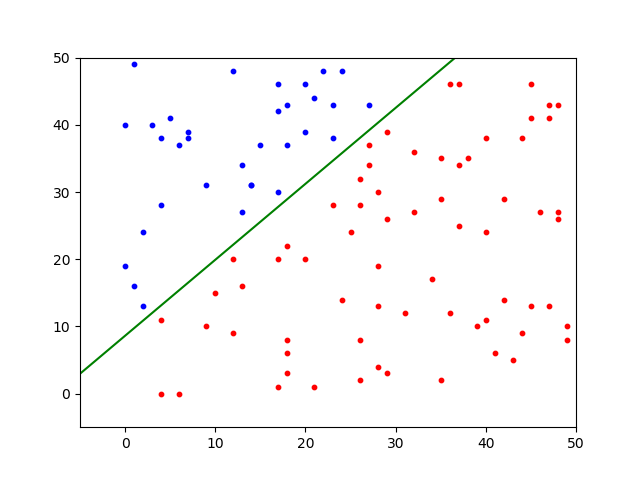
\includegraphics[width=10cm]{../results/linear.png}
    \end{center}
\end{figure}
次にカーネルトリックを用いて,sample\_circle.txtにSVMを実装した.ガウスカーネルを用いた結果についてはFigure 2,多項式カーネルを用いた
結果についてはFigure 3である.ここでガウスカーネルでは$\sigma=10$とした.先ほどと色が変わってしまったが,黒の曲線が識別器の
境界を示しており,正しく分類できていることが図から読み取れる.\par
\begin{figure}[htpb]
    \begin{minipage}{0.50\hsize}
        \begin{center}
            \caption{ガウスカーネル}
            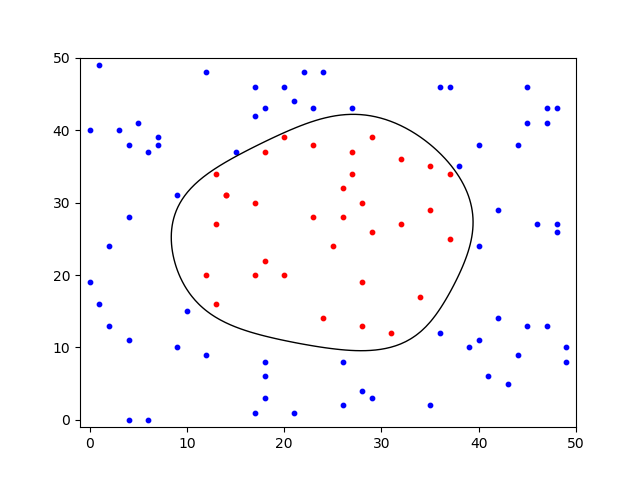
\includegraphics[width=70mm]{../results/gaussian_sigma=10_circle.png}
        \end{center}
    \end{minipage}
    \begin{minipage}{0.50\hsize}
        \begin{center}
            \caption{多項式カーネル}
            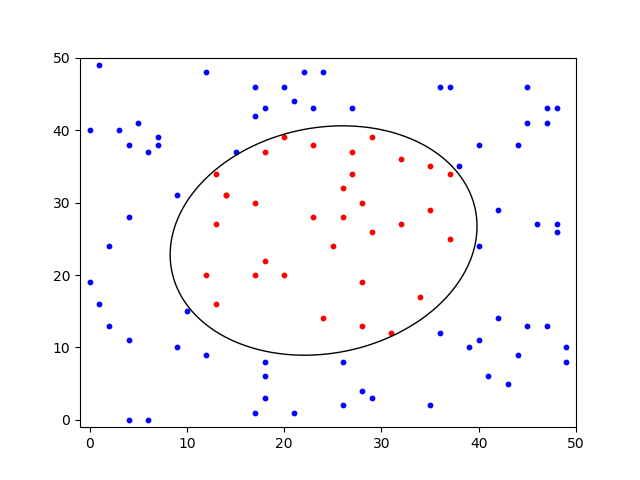
\includegraphics[width=70mm]{../results/poly_circle.png}
        \end{center}
    \end{minipage}
\end{figure}
最後にガウスカーネルのパラメータ$\sigma=5$として実行した結果がFigure 4である.\\
\begin{figure}[htbp]
    \begin{center}
        \caption{ガウスカーネル($\sigma$変更)}
        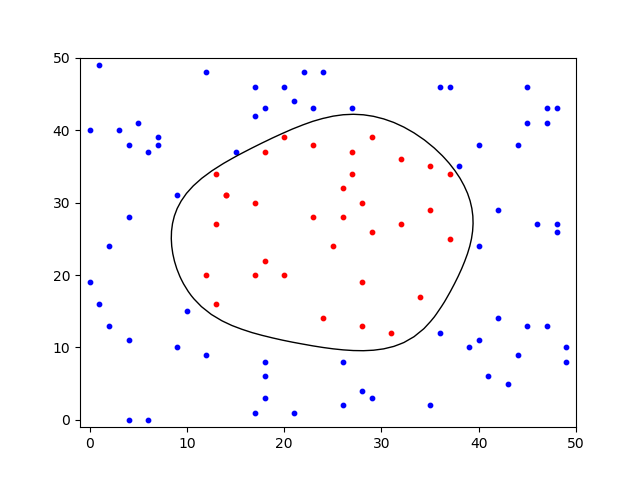
\includegraphics[width=8.5cm]{../results/gaussian_sigma=5.png}
    \end{center}
\end{figure}

\subsection{交差検定結果}
まずsample\_linear.txtに関して交差検定を行ったところ,データ分割数をいかなる値,例えば最小の2にしても正解率100\%であった.
sample\_circle.txtに対して検定を行った結果を下のTable 2にまとめる.\\

\begin{table}[htb]
    \begin{center}
        \caption{コマンド使用方法}
        \begin{tabular}{|c|c|c|c|} \hline
        カーネル & 分割数 & $\sigma$の値 & 結果(平均) \\ \hline \hline
        ガウス & 5 & 10 & 89\% \\ \hline
        ガウス & 10 & 10 & 90\% \\ \hline
        ガウス & 5 & 5 & 91\% \\ \hline
        ガウス & 10 & 5 & 91\% \\ \hline
        多項式 & 5 & - & 96\% \\ \hline
        多項式 & 5 & - & 96\% \\ \hline
        \end{tabular}
    \end{center}
\end{table}
参考までに,ガウスカーネルを用いて分割数5とした場合で正答率が最も悪い80\%であった時のグラフは,以下のFigure 5のようになった.

\begin{figure}[htbp]
    \begin{center}
        \caption{参考画像}
        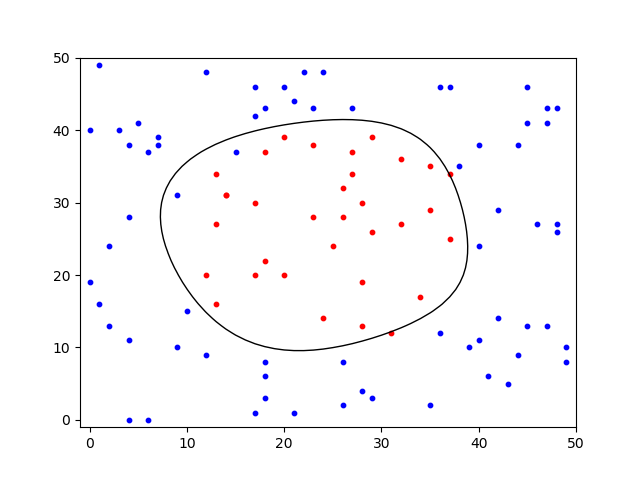
\includegraphics[width=8.5cm]{../results/gaussian_sigma=10_2703_accuracy=0_8.png}
    \end{center}
\end{figure}

\section{考察}
評価結果から自明なように,sample\_linear.txtに対しては,非常に精度の高い分類が可能であった.
分割数を変更しても正解率は100\%であったのは,サンプルデータが非常に綺麗に分類できるものであったということも理由と考えられる.
sample\_circle.txtに対しても,交差検定を実装しても正解率が高く図を見ても正しく分類できたと言える.
またガウスカーネルにおいて,$\sigma$の値を小さくすると境界線の凹凸が激しくなり,逆に大きくすれば滑らかな曲線が描写される.
多項式カーネルにおいては,カーネルの定義式の性質上楕円のような境界線が描かれていることがわかった.こちらのサンプルデータもそもそもが綺麗なデータであったので,
結果の精度も良かったと考えられる.

\section{感想}
シグモイドカーネルの実装でパラメータをどのような値にすれば良いのかよくわからなかったので,実装できなかったのが残念だった.
またサンプルデータだけでなく,他のデータにも適用させたかったが,時間があまりなくて試すことができなかった.最終課題では満足のいくところまで実装をやりきりたい.

\end{document}